\documentclass[a4paper]{article}

\usepackage{color}
\usepackage{url}
\usepackage[utf8]{inputenc}
\usepackage{graphicx}

\usepackage[english,serbian]{babel}

\usepackage[unicode]{hyperref}
\hypersetup{colorlinks,citecolor=green,filecolor=green,linkcolor=blue,urlcolor=blue}


\begin{document}
\title{VAR tehnologija\\ \small{Seminarski rad u okviru kursa\\Tehničko i naučno pisanje\\ Matematički fakultet}}

\author{Luka Šešelja\\ luka.seselja123@gmail.com \and Ognjen Arsenijević\\ ogiarsenijevic1@gmail.com \and Ognjen Radivojević\\ radivojevicognjen03@gmail.com}
\date{20.~novembar 2022.}
\maketitle

\begin{abstract}
    
\end{abstract}

\tableofcontents

\newpage

\section{Uvod}
\textbf{VAR tehnologija} (eng. ~{\em Video Assistant Referee}) je revolucionarna tehnologija koja se koristi u fudbalu i omogućava sudijama da koriste video snimke tokom utakmice kako bi doneli pravednu odluku u slučaju nejasnih situacija na terenu. Ova tehnologija je  zvanično uvedena u fudbal 2018. godine, a od tada se koristi u mnogim fudbalskim ligama i takmičenjima širom sveta.

VAR tehnologija se smatra velikim napretkom u sportu, jer omogućava da se sudijske odluke donesu na temelju činjenica i da se smanje greške sudija. Međutim, takođe je izazvala neke kontroverze i rasprave o tome koliko se tehnologija treba koristiti u sportu i koliko bi uticaja trebalo da ima u odlučivanju o rezultatu utakmice.

\section{Istorija}
Ideja o upotrebi video tehnologije u fudbalu počela je da se razvija 2010. godine, u okviru projekta "Refereeing 2.0" u Holandiji. \cite{istorija} Sistem je testiran tokom sezone 2012-13. godine u okviru Eredivizije (hol. ~{\em Eredivisie, u prevodu Divizija časti ili Premijer liga}), najviše profesionalne fudbalske lige u Holandiji.

Nakon toga, VAR tehnologija je nastavila da se razvija i unapređuje kroz prijateljske utakmice,a prvi put je uživo testiran u julu 2016. godine. 

Prva profesionalna utakmica u kojoj je VAR testiran bila je zvanična utakmica prvog kola KNVB kupa 2016. godine. Ovaj meč je bio prvi meč u kom se pojavio ”monitor pored terena“. On se koristi kada sudija na terenu želi da proveri određene sporne situacije. Omogućava mu takođe ponovni pregled tih situacija snimljenih različitim kamerama iz više različitih uglova, kako bi mogao da donese ispravnu odluku.

Pored navedenih, tokom sledeće dve godine obavljena su brojna testiranja i zahvaljujući njima, Var sistem je konacno implementiran u zvanična pravila fudbala u martu 2018. godine.

Od tada se VAR tehnologija koristi u mnogim fudbalskim ligama i takmičenjima, uključujući i Ligu šampiona i Svetsko prvenstvo. Prvo Svetsko prvenstvo na kom je bila upotrebljena je Svetsko prvenstvo u Rusiji 2018. godine. \cite{prvenstvo}

\section{Primena VAR tehnlogije u praksi}
\subsection{Slucajevi u kojima se koristi VAR tehnologija}
Pravila igre ostavljaju prostor za tumačenje i istraživači su pokazali da na sudije mogu uticati spoljašnji faktori kao što su buka publike(Nevill et al.,2002), prednost domaćeg terena(Unkelbach \& Memmert, 2010), kao i prethodne odluke(Plessner \& Betsch, 2001). Odluke koje sudije donose stoga nisu 100\% ispravne, te je VAR osmišljen i uveden kako bi vršio korekciju jasnih i očiglednih grešaka u četiri slučaja:
\begin{itemize}
\item Gola ili prekršaja koji dovodi do gola
\item Penala ili prekršaja koji dovodi do penala
\item Dodele direktnog crvenog kartona
\item Greške pri identifikovanju igrača
\end{itemize}

VAR može da inteveniše kada je pogrešna odluka rezultat jednog ili više koraka u procesu donošenja odluke(Plessner \& Haar, 2006):

Pažnja i percepcija (npr. kada je promašen ozbiljan incident u kaznenom prostoru ili sudija nije video da li je lopta prešla gol liniju ili ne);

Obrada informacija i kategorizacija (npr. kada je ozbiljna faul igra pogrešno kategorisana kao žuti umesto kao crveni karton);

Odgovor na ponašanje (npr. kada je incident dobro shvaćen i kategorisan, ali je žuti karton dat pogrešnom igraču, što je označeno kao pogrešan identitet).
\subsection{Podešavanje kamere}
Sudijski tim video pomoćnika ima pristup četrdeset dve kamere za emitovanje, od kojih su osam super usporene (eng.~{\em super slow motion}) i četiri ultra usporene (eng.~{\em ultra slow motion}). Usporene reprize se uglavnom koriste za činjenične situacije, na primer, da bi se identifikovala tačka kontakta fizičkog prekršaja ili pozicija prekršaja. Ponavljanja normalne brzine se koriste za subjektivne procene, na primer, da bi se utvrdio intenzitet prekršaja ili da li je igra rukom kažnjiva. Pored kamera za emitovanje, VAR tim ima pristup fidovima kamere koje koristi polu-automatska ofsajd tehnologija (eng.~{\em semi-automated offside technology}).


\begin{figure}[h!]
\begin{center}
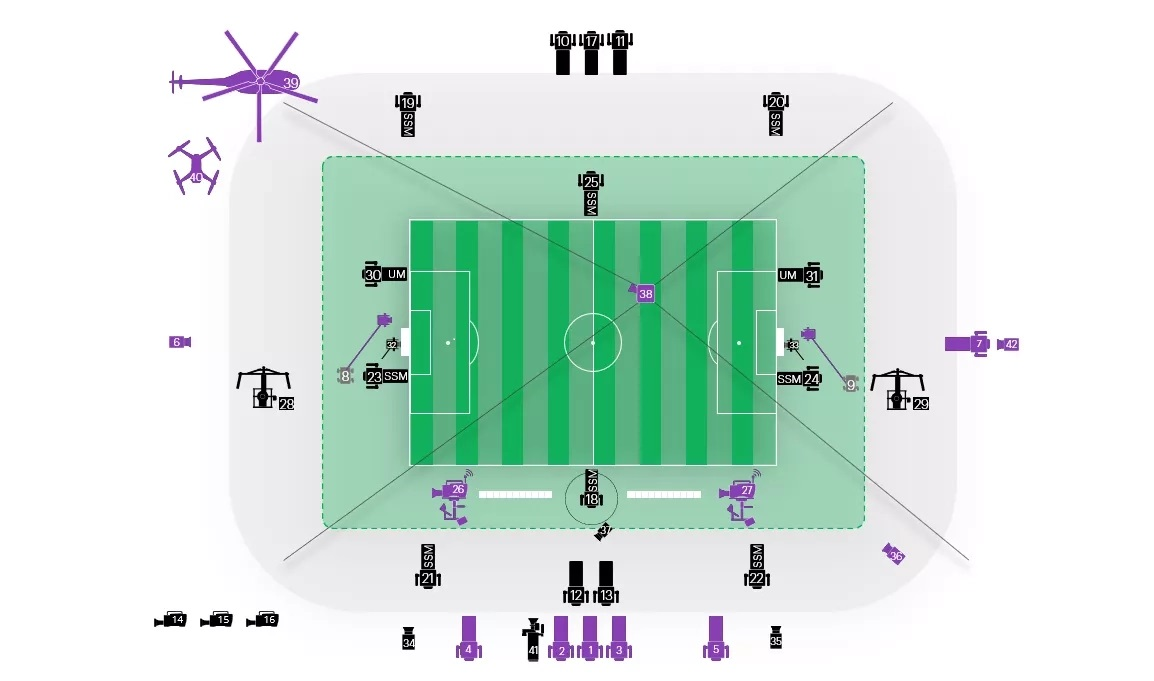
\includegraphics[scale=0.35]{Var sistem.jpeg}
\end{center}
\caption{Kamere}
\label{fig:kamere}
\end{figure}

Na slici \ref{fig:kamere} prikazan je raspored kamera na terenu u okviru VAR sistema.

\subsection{VAR tim}
VAR tim se sastoji od: 
\begin{itemize}
\item VAR sudije(eng.~{\em video assistant referee}) koji gleda glavnu kameru na gornjem monitoru i proverava ili pregleda incidente na četvorostrukom monitoru. Štaviše, VAR je odgovoran za vođenje VAR tima i komunikaciju sa sudijom na terenu.
\item Prvog asistenta VAR sudije (AVAR1) koji se koncentriše na glavnu kameru i obaveštava VAR sudiju o igri uživo ako se incident proverava ili pregleda.
\item Drugog asistenta VAR sudije (AVAR2) koji je zvaničnik za video meč sa iskustvom pomoćnog sudije i nalazi se na ofsajd stanici i proverava sve potencijalne ofsajd situacije, uz pomoć poluautomatizovane ofsajd tehnologije, kako bi ubrzao VAR proveru i proces pregleda.
\item Trećeg asistenta VAR sudije(AVAR3) koji se fokusira na kanal TV programa, pomaže VAR-u u proceni incidenata i obezbeđuje dobru komunikaciju između VAR-a i AVAR2 koji se nalazi u ofsajd stanici.
\item Sudijske oblasti za pregled (eng. ~{\em Referee review area (RRA)}) je jasno označeno područje koje sadrži ekran koji omogućava sudiji da pregleda incidente. Nalazi se pored terena, u blizini tehničkih zona.
\end{itemize}

\section{Preciznost provera i statistika} 
\subsection{Preciznost odluka} 
Ispravnost sudijske odluke podeljena je na dva dela: tačnost početne odluke(odluke pre VAR provere) i tačnost konačne odluke(odluke posle VAR provere). Preciznost sudijskih odluka se meri u procentima i predstavlja procentualni odnos slaganja sudijskih odluka sa odlukama nacionalnog sudijskog komiteta. 

\subsection{Trajanje provera i pregleda} 
Trajanje provere se odnosi na vreme potrebno VAR timu da proveri spornu situaciju i utvrdi da li treba da se izvrši pregled. Pregled glavnog sudije na terenu počinje kada rukama pokaže oblik TV ekrana i završava se kada donese konačnu odluku. Prema VAR protokolu, pregled situacije može da se izvrši samo komunikacijom sa VAR sobom, ili se može dopuniti pregledom glavnog sudije na terenu. Trajanje provere u VAR sobi meri se odvojeno od trajanja pregleda na terenu.

\subsection{Statistička analiza}
Na osnovu ispitanih šansi za tačne početne i konačne odluke koristeći model logističke regresije, u ovoj analizi je zaključeno da svaka situacija jeste doprinela i početnoj i konačnoj (nakon potencijalne intervencije VAR-a) odluci sudije. Odluke nisu bile statistički nezavisne jer su sudije imale više od jedne odluke. Da bi se važio ovaj poslednji faktor, korišćen je model nasumičnih efekata. 


\subsection{Preciznost odluka} 
Bilo je ukupno 9732 provere u 2195 utakmica. Sveukupno, 638 situacija je svrstano u sivu zonu, odnosno odluke za koje ne postoji jasna referentna odluka od strane nacionalnog sudijskog komiteta (tj. može se podržati više odluka). Bilo je 99 pregleda za incidente u sivoj zoni, a sudija je promenio prvobitnu odluku 44 puta (7\% svih odluka)
Prvobitna odluka sudije bila je tačna u 8376 od 9094 čiste situacije, što je donelo tačnost odluke od 92,1\%. Nakon intervencije VAR-a, 8942 od 9094 situacije su bile ispravne, što je dalo procenat tačnosti od 98,3\%.  

U 585 od 718 incidenata sa pogrešnim početnim odlukama (81,5\%), odluka je preispitana i 577 ovih odluka je ispravljeno. 

U 111 od 8376 incidenata sa ispravnim početnim odlukama (1,3\%), odluka je preispitana i 11 od njih je preinačeno u netačnu odluku. 

Srednje trajanje 9732 provere(u proseku 4,4 provere po meču) bilo je 22,0 sekunde. Srednje trajanje svih provera tokom meča bilo je 110,0 sekundi. 
Ukupno, 795 od ovih provera rezultiralo je pregledom (0,36 pregleda po meču u proseku), tačnije 534 su bile provere glavnog sudije na terenu sa srednjim trajanjem od 62,0 sekunde i 261 je bila samo VAR procena u sobi sa srednjim trajanjem od 15,0 sekundi. 

Bilo je 1544 utakmice bez pregleda(70,3\% svih utakmica); 530 utakmica sa samo jednim pregledom(24,2\% svih mečeva); 103 meča sa 2 pregleda (4,7\% svih mečeva); 15 utakmica sa 3 pregleda (0,7\% svih mečeva); 2 meča sa 4 pregleda (0,1\% svih mečeva) i 1 meč sa 6 pregleda (0,1\% svih mečeva).

Najveći udeo provera imali su incidenti sa crvenim kartonom (39,3\%), zatim kazneni incidenti (33,4\%), golovi (27,1\%) i pogrešan identitet (<1\%). Incidente sa penalima (43,9\%) imali su najveći udeo pregleda, zatim golovi (32,5\%), incidenti sa crvenim kartonom (22,5\%) i pogrešan identitet (1,1\%).

U slučaju pregleda, sudija ima mogućnost da promeni prvobitnu odluku. Bilo je 76 dodatnih penala (164 dosuđenih penala; 88 poništenih), 126 dodatnih crvenih kartona (132 dodeljena crvena kartona; 6 crvenih kartona poništenih) i 114 golova manje (61 gol; 175 poništenih golova) zbog intervencija VAR-a.



\addcontentsline{toc}{section}{Literatura}
\appendix

\iffalse
\bibliography{seminarski} 
\bibliographystyle{plain}
\fi

\begin{thebibliography}{9}

\bibitem{istorija} \em{Video assistant referee}. (2022, December 16). In Wikipedia. \url{https://en.wikipedia.org/wiki/Video_assistant_referee}  

\bibitem{prvenstvo} Gidget Alikpala. \em{Qatar 2022 World Cup: What is the VAR and when is it used?} (Diario AS, 2022, December 16). \url{https://en.as.com/soccer/qatar-2022-world-cup-what-is-the-var-and-when-is-it-used-n-2/}

\bibitem{} Jochim Spitz, Johan Wagemans, Daniel Memmert, A. Mark Williams, Werner F. Helsen. \emph{Video assistant referees (VAR): The impact of technology on decision making in association football referees}. Routledge, 2021. on-line at: https://doi.org/10.1080/02640414.2020.1809163

\bibitem{} Nevill, Alan and Balmer, Nigel and Williams, Andrew. \\ \emph{The Influence of Crowd Noise and Experience upon Refereeing Decisions in Football}. Psychology of Sport and Exercise, 2002. on-line at: https://www.researchgate.net/publication/222697584

\bibitem{} Henning Plessner, Tilmann Betsch. \emph{Sequential Effects in Important Referee Decisions:The Case of Penalties in Soccer}. Human Kinetics Publishers, Inc, 2001 on-line at: https://www.researchgate.net/publication/23753046


\end{thebibliography}

\end{document}
